\clearpage\secrel{\uF\ for microcontrollers}\secdown\label{micro}

This chapter contains sample of tiny \F\ system can be used on embedded
devices built with any microcontrollers or SoCs having \emph{more then 8K RAM,
UART} or any serial/packet/network interface:
\begin{description}
\item[interactive control shell] can use any serial or packet interface\\
UART, Telnet, scripts on SD card, GSM/SAT modem,\ldots
\item[scripting engine] with optional on-board assember/compiler
\item[programming system] based on tight RAM-effective bytecode\\
highly configurable, multitasking, custom user VM instructions doing complex
things in one command,\ldots
\end{description}

\clearpage\secrel{Build from source (files)}

\begin{tabular}{l l}
Makefile & build scripts \\
.gitignore & files masks for generated and temp files (for git) \\
micro.c & Virtual Machine source code\\&extra portable, written in strict
ANSI C'89\\
compiler.lex & compiler source code (flex/\cpp) \\
FORTH.uF & \F-system source code\\&written in \term{compiling script} syntax\\
\end{tabular}

\bigskip\noindent
Install MinGW or GNU toolchain, and build it using
\begin{lstlisting}
$ cd ~/o/micro ; [mingw32-]make
\end{lstlisting}

\clearpage\secrel{Run system}
You will get few .exe\note{.exe required for Windows, and have no matter for
Linux} files in current directory:

\medskip\noindent
\begin{tabular}{l l}
uFORTH.exe & emulator to run on your host system \\
compiler.exe & simple bytecode compiler using \F-like script \\
FORTH.bc & demo system compiled into bytecode
\end{tabular}

\medskip\noindent
\verb|.bc| file is optional: resulting \verb|uFORTH.exe| was built as
full-functional standalone executable, and all required bytecode was
in-compiled. But \emph{you can run your own programs in .bc files} as:
\begin{lstlisting}
$ ./compiler.exe < YourProgram.uF > compiling.log
$ ./uFORTH.exe YourProgram.bc
\end{lstlisting}

\clearpage\secrel{Low-level architecture}

\emph{This system primarily targeted for tiny embedded devices},\\
so \textcolor{red}{u\F\ is 16 bit only}. To do it usable toy on large
computers\note{Android is good candidate to play on mobile phone} it is not
required to be big\ --- remember old friendly home computers having not more
than 64K of RAM. In fact, \textcolor{red}{\F\ blew the best platform for
this language}: ZX Spectrum and Commodore 64.

\smallskip\noindent
\begin{tabular}{l l l}
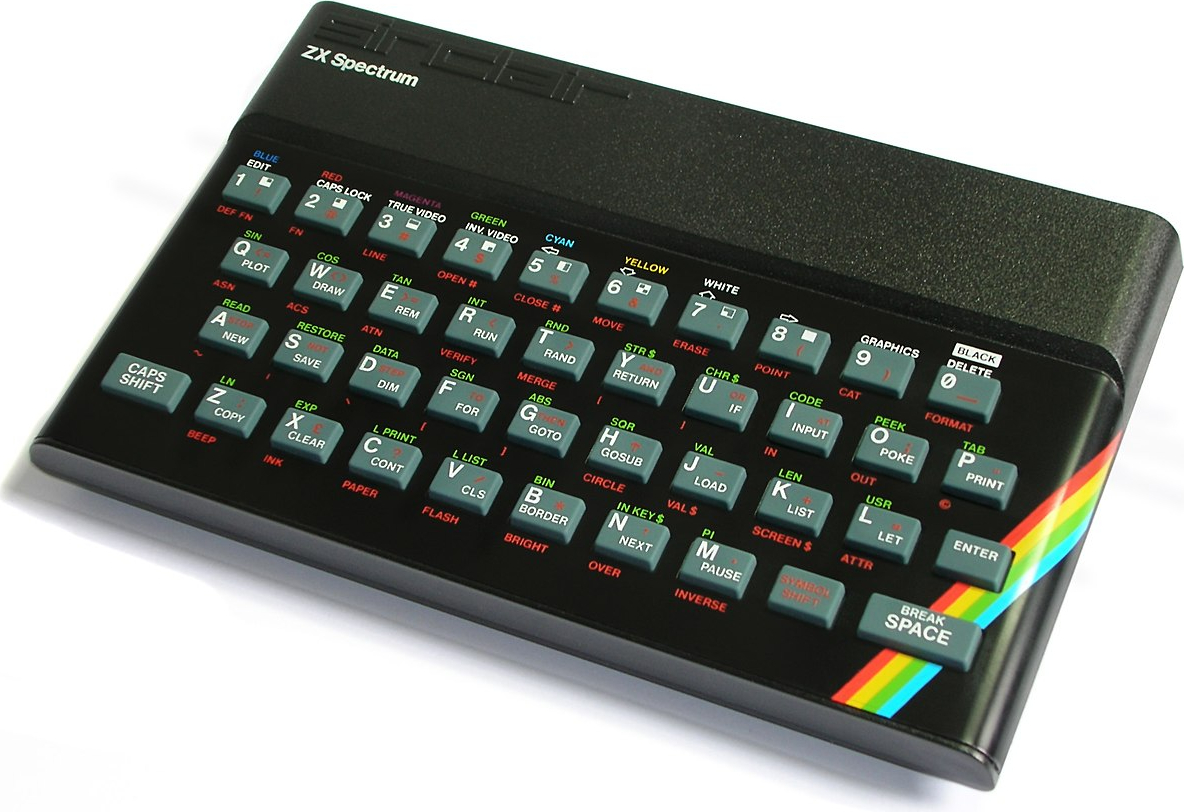
\includegraphics[height=0.35\textheight]{img/ZX48.jpg} &
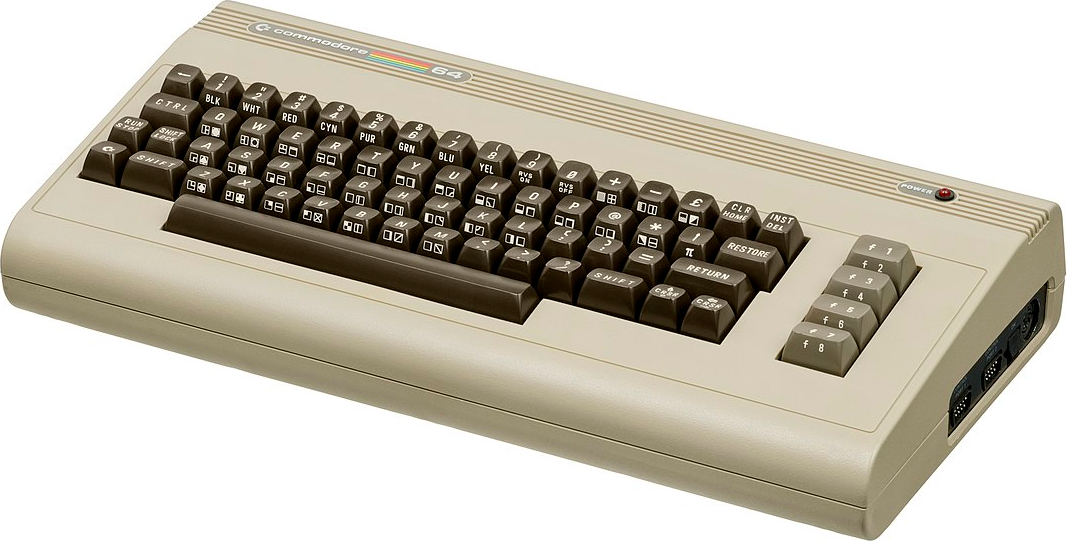
\includegraphics[height=0.35\textheight]{img/C64.jpg} &
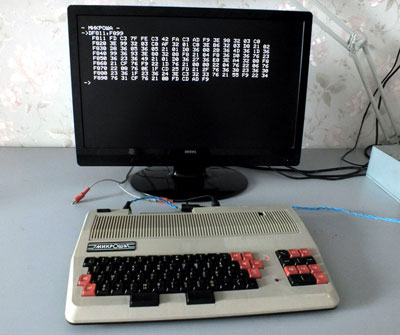
\includegraphics[height=0.35\textheight]{img/microsha.jpg} \\
\end{tabular}
\clearpage

\noindent
This tiny computers was totally (!) conformant to \F:
\begin{itemize}[nosep]
  \item few RAM starting from 16K, and not more then 64K\\
  (some latest models had 128K)
  \item tiny 8bit cheap processor: i8080, Z80, 6502
  \item user must be able to program it using ROM firmware\\using easy
  high-level programming language
  \item real programs must be written in assembly because of lack of RAM
  and CPU power
  \item direct access to hardware: strange framebuffer and i/o ports
\end{itemize}
BASIC was selected for learning, but \emph{all these computers allow to replace
ROM} chip or use external pluggable ROMs. And FORTH fails the same way as
SmallTalk: \textcolor{red}{price kills the language feature}.

\clearpage

\noindent
Notably, this \term{deskboard computer formfactor} still \emph{can be accepted
by consumer market}. In early days of hobby home computing, the most annoying
problem was keyboard quality: they were ugly. Modern technologies allow making a
good quality keyboard with embedded SoC power enough to process multimedia
without any lags and do good gaming graphics in hardware level. Large casing
lets to use modern multicore mobile SoCs from MTK and AllWinner with OpenGL
and large RAM, without any problems of overheating. Backside able to carry all
required interfaces: Ethernet, HDMI+VGA, and huge USB hub.
Other variant is \emph{extra cheap computers}: STM32F7 MCU family
have enough interfaces and computing power to be good in this old style cheap
consoles.

\clearpage

\begin{lstlisting}[language=C]
/* sizes of statically allocated structures */
#define Dsz 0x10
#define Rsz 0x100
#define Msz 0x1000

void VM() {}	/* virtual machine startup */

#ifdef EMULATOR
/* this code will be compiled only for emulator */
int main() { VM(); return 0; }
#endif
\end{lstlisting}
\begin{lstlisting}[language=C]
#include <stdint.h>						/* std.includes */
#ifdef EMULATOR ...	/* for emulator mode only */

/* set 16/32 bit mode
	CELL is machine word for FORTH systems */
#define  CELL  int16_t /* light microcontrollers */
#define UCELL uint16_t

/* data stack */
 CELL D[Dsz]; uint16_t Dp=0; /*[D]ata [p]ointer*/
/* return stack */
UCELL R[Rsz]; uint16_t Rp=0; /*[R]eturn [p]ointer*/
\end{lstlisting}


\clearpage
\secrel{Vocabulary structure}\label{uvocab}

\begin{tabular}{l l l}
LFA & UCELL & Link Field Area \\
NFA & CNTSTR & Name \\
AFA & BYTE & Attribute (IMMED flag) \\
CFA & \ldots & Code \\
PFA & (optional) & Parameter for vairables/constant/\ldots\\
\end{tabular}

First word can be FORTH or any name (of your application for example) does
nothing. Last defined word will be entry point.

\clearpage\secrel{$\mu$Compiler}\label{ucompiler}

uCompiler into bytecode was written as standalone application in flex/bison. It
implements some sort of portable assembly: resulting code is extra compact
comparing to most known real machine code formats. The uCompiler has no ability
to execute code in compile time, so you can't use some tricks available in
any generic \F\ system. You can solve this problem by extending the compiler
or syntax parser grammar let you adapt input language for your needs.

\clearpage\secrel{\uF\ in JavaScript}\secdown

In file
\href{https://github.com/ponyatov/o/raw/master/micro/uFORTH.html}{/o/micro/uFORTH.html}
you can found \uF\ implementation written in \js. You can use it as \emph{microWeb platform} \ref{uweb}\ or just give it as advertisement demo to your colleague to show how device interface will look like for user
connects via terminal.

\secup

\secup
